
We fix throughout a time horizon $T>0$ and a probability space $(\Omega, \calF, \Q)$.  
Let us assume that the price vector $S = (S_t)_{t\in [0,T]}$, $S_t = (S_{t,1},...,S_{t,d}) \in \R_{+}^d$  is a c\`adl\`ag  process. 
We adopt the notation $\SSS_t = (S_u)_{u\in [0,t]}$ so that for 
$\Q-$almost every $\omega \in \Omega$,  $\SSS(\omega)$ belongs to $ \Lambda := \bigcup_{t\in [0,T]} \Lambda_t$ with the  Skorokhod spaces $\Lambda_t := \calD([0,t],\R^d_+).$ 

So far, it is not assumed that $S$ is a Markov process. Indeed, the dynamics of $S$ may depend on exogenous factors $\calV_t = (\calV_{t,1},...,\calV_{t,l}) \in \R^l$ (e.g. stochastic volatility, interest rate, volume, etc). However, we require that the enlargement $(S,\calV)$ is a c\`adl\`ag Markov  process with respect to its natural filtration, which we denote by $\F$. The probability space is henceforth filtered with $\F$. 

 
Moreover, let  $B=(B_t)_{t\in [0,T]}$ be the money market account and $D_{t,u} = \frac{B_t}{B_u}$ the 
discount factor over the interval $ [t,u]$. We  impose the mild restriction that $D_{t,u} \in [0,1]$ for all $0\le t \le u \le T$, i.e. $B$ is non-decreasing. This amounts to saying that interest rates are non-negative. 

\subsection{Optimal Stopping}
We  associate to any reward functional $\Phi: \Lambda \to \R$ and subset $\calT \subseteq [0,T]$ the \textit{optimal stopping problem}, 
\begin{equation}\label{eq:OS}
\underset{\tau \, \in \, \vartheta(\calT)}{\text{sup}} \ \E^{\Q}[D_{0,\tau}\, \Phi(\SSS_{\tau})],
\end{equation} 
where $\vartheta(\calT)$ is the set of $\F-$stopping times taking values in $\calT$. Notice that the factors $ (\calV_{\cdot,1},\ldots, \calV_{\cdot,l})$ (if any) do not appear in the payoff. We nevertheless observe $\calV$ (as $\F$ is the natural filtration of $\bar{S}$) which may influence our stopping decision. 

To make $\eqref{eq:OS}$ nontrivial,
it is often assumed that $\sup_{t \in \calT} \Phi(\SSS_{t}) \in L^1(\Q)$; see \cite{PeskirShiryaev}. Solving the optimal stopping problem without further assumptions on $\Phi$ proves hard as 
$(S,\Phi(\SSS),\calV)$ may fail to be a Markov process. 

To circumvent this issue, we impose the following condition on $\Phi$. 
\begin{asm}\label{asm:enlargement}
There exists $k\in \N$ and a vector-valued functional $\Upsilon: \Lambda \to \R^k$ such that
\begin{enumerate}
\item $Y := (\Upsilon(\SSS_t))_{t\in [0,T]}$ has c\`adl\`ag trajectories $\Q-$a.s. 
    \item $X := (S,Y,\calV)$ is a Markov process with state space $\calX \subseteq  \R^d_+ \times \R^{k} \times \R^{l}$.
    \item  $\Phi(\SSS_t) = \varphi(X_t)$ for some function $\varphi:\calX \to \R$ such that  $ \forall \ x=(s,y,\nu) \in \calX$,  $\varphi(x)$ does not depend on $\nu$.
\end{enumerate}
\end{asm}

When $\Phi$ is path-independent, the above assumptions are not needed and we simply set $k=0$ and $X=(S,\calV)$. With a slight abuse of notation, we may occasionally write $\varphi(x)=\varphi(z)$, where $x=(z,\nu)$ and  
\begin{equation} \label{eq:Z}
    z\in \calZ := \{(s,y) \in \R_+^d \times \R^k \ | \ (s,y,\nu) \in \calX \text{for some } \nu \in \R^k\}.
\end{equation} 
When $k=0$, we  may even use $\varphi(x)$ and $\varphi(s)$ interchangeably.  % and use $\Phi$ or $\varphi$ interchangeably. 
Problem $\eqref{eq:OS}$ can therefore be reformulated as follows:
\begin{equation}\label{eq:OS2}
\underset{\tau \, \in \, \vartheta(\calT)}{\text{sup}} \ \E^{\Q}[D_{0,\tau}\, \varphi(X_{\tau})].
\end{equation} 
Having now a Markovian framework, we can introduce the \textit{value function} associated to $\eqref{eq:OS2}$, that is
\begin{equation} \label{eq:valueFct}
v(t,x):= \underset{\tau \, \in\,  \vartheta(\calT_{\!t})}{\text{sup}} \
\E^{\Q}\! \left[ D_{t,\tau}\ \varphi(X^{t,x}_\tau)\ \right],\quad (t,x)\in [0,T]\times \calX,
\end{equation} %\underset{\tau \in \llbracket t,T \rrbracket}{\text{ess sup}}
with $\calT_{\!t} = \calT \cap \ [t,T]$ and $X^{t,x} = (X_u^{t,x})_{u\in [t,T]}$ denotes the forward-starting process such that $X^{t,x}_t= x \in \calX$.  We stress that  $\E^{\Q}\! \left[ D_{t,\tau}\ \varphi(X^{t,x}_\tau)\ \right]$ is understood as $\E^{\Q}\! \left[ D_{t,\tau}\ \varphi(X_\tau)\ | \ X_t= x\right]$.  %and the simplified notation $\E_{t,s}^{\Q}[\cdot]=\E^{\Q}[\cdot\,|\, S_t=s].$ 
The optimal stopping problem  $\eqref{eq:OS2}$ therefore consists of finding $v(0,\cdot)$.

When $\Q$ is a risk-neutral measure, $v$ is construed in finance as the price function of an \textit{option}  (or \textit{contingent claim}) with payoff $\varphi$ and exercise dates $\calT$. We will stick to this interpretation throughout this section and beyond.
Options are subdivided into roughly three families  characterized by their exercise style. More specifically, an option is called 
% \begin{itemize}
%     \item[(i)] \textit{European} if $\calT = \{T\}$,
%     \item[(ii)] \textit{Bermudan} if $\calT = \{t_1,\ldots,t_n\}$ where $0\le t_1 < \ldots < t_n \le T $, $n\in \N$,
%     \item[(iii)] \textit{American} if $\calT = [0,T]$.
% \end{itemize}
(i) \textit{European} if $\calT = \{T\}$, (ii) \textit{Bermudan} if $\calT = \{u_1,\ldots,u_n\}$, $0\le u_1 < \ldots < u_n \le T $, $n\in \N$, or (iii) \textit{American} if $\calT = [0,T]$. It is often assumed that any claim permits the holder to exercise at maturity, i.e. $T\in \calT$. In view of $\eqref{eq:valueFct}$, this ensures  that $v^{\text{European}} \le v^{\text{Bermudan}} \le v^{\text{American}} $, with the obvious notation.  Note that for European options, we simply have $v^{\text{European}}(t,x)= \E^{\Q}\! \left[ D_{t,T}\ \varphi(X^{t,x}_T)\ \right]$. We will therefore turn our attention to options of Bermudan or American type.

Although promising a continuum of exercise dates is idealistic, American options remain the most common product on derivatives markets and the most challenging from a mathematical standpoint. For options of American type, one is  forced to approximate the contract by a Bermudan option whose exercise dates cover $[0,T]$ (see \citet{Guyon}). The price is thereafter easily computed using Dynamic Programming. %Also observe that American contracts are idealistic as financial markets still operate in discrete time. However, American options present  great challenges and elegance from a mathematical standpoint.

%the function $\varphi$ is the \textit{payoff} of an option with early exercise and $v$ is its \textit{price}. 
It is clear that a rational agent would stop (or exercise) the contract at  $t\in \calT$ 
as soon as $v(t,x) \le \varphi(x)$. On such occasions, we in fact have $v(t,x) = \varphi(x)$ since $t$ is itself a stopping time and $\varphi(x) = \E^{\Q}\! \left[ D_{t,t}\ \varphi(X^{t,x}_t)\ \right] \le v(t,x)$. 
This brings us to the following definition. 
\begin{definition}
The \textit{stopping region} is defined as $\calS := \prod_{t\in \calT} \calS_t \subseteq \calT \times \calX$, with  the  $t-$sections 
\begin{equation}\label{eq:stopRegion}
    \calS_t:= \left\{ x \in \calX\ | \
v(t,x)=\varphi(x)\ \right\}, \quad t\in \calT\!.
\end{equation}
%When it is not optimal to stop, we are in 
Its complement 
is the 
the \textit{continuation region}, namely
$$\calC =\prod_{t\in \calT} \calC_t, \quad \calC_t:= \left\{ x \in \calX\ | \
v(t,x) > \varphi(x)\ \right\}. $$
\end{definition}

Notice in particular that $\calS_T=\R^d_+$ as the payoff and value function coincide at maturity.
\begin{remark}
The partition of $\calX$ into the stopping and continuation region is only made for dates at which the option can be exercised. Equivalently, one could have defined 
$\calS = \prod_{t\in [0,T]} \calS_t \subseteq [0,T]\times \calX$ ($\calC = \prod_{t\in [0,T]} \calC_t$) and set $\calS_t =\varnothing$ ($\calC_t =\calX$) whenever $t\notin \calT$. 
\end{remark}
As every Borel measurable subset $\calU \subseteq \calT \times \calX$ is paired with the hitting time $$\tau(\calU) := \inf\{t\in \calT \ | \ (t,X_t) \in \calU \}\wedge T,$$
it is easily seen that
\begin{equation}\label{eq:subset}
   v(0,X_0) =\underset{\calU \, \subseteq \, \calT \times \R^d_+}{\text{sup}} \, \E^{\Q}[D_{0,\tau(\calU)}\, \varphi(X_{\tau(\calU)})].  
\end{equation}
Indeed, $v(0,X_0)$ clearly dominates the right hand side of $\eqref{eq:subset}$, while  $\tau(\calS)= \inf\{t\in \calT \ | \ v(t,X_t)= \varphi(X_t) \} \wedge T$ is known to be the (smallest)   stopping time maximizing $\eqref{eq:OS}$; see, e.g., Theorem 2.2 in  \citet{PeskirShiryaev}. 

\subsection{Free Boundary}

The first connection between American options and free boundary problems is due to
\citet{mcKean}, a decade before the celebrated Black \& Scholes formula. We here state the result in a quite general framework. In what follows, we suppose that $X$ is in addition a Feller process. The infinitesimal generator of $S$ is denoted by $\calL: \calD_{\calL} \to \calC_0(\calX)$, where $\calD_{\calL}$ is its domain and $\calC_0(\calX) \subseteq \calC(\calX)$ the family of  continuous functions  vanishing at infinity.  
Moreover, we assume that the money market account is a deterministic process and write $$\hat{\varphi}(t,x):= D_{0,t}\ \varphi(x), \quad \hat{v}(t,x):= D_{0,t} \ v(t,x),$$
for the discounted reward and value function, respectively. As $D_{0,t}D_{t,u}=D_{0,u}$ for $0\le t \le u \le  T$, we simple have   $\hat{v}(t,x)= \sup_{\tau \, \in\,  \vartheta(\calT_{\!t})} \ \E^{\Q}\! \left[ \,  \hat{\varphi}(\tau, X^{t,x}_\tau)\ \right].$ We recall that the process 
$$\hat{v}(t,X_t)= \underset{\tau \, \in\,  \vartheta(\calT_{\!t})}{\text{ess sup}} \ \E^{\Q}\! \left[ \,  \hat{\varphi}(\tau, X^{t,x}_\tau)\ \right]\big |_{x=X_t}, \quad t \in [0,T],$$
is the \textit{Snell envelope} of $\hat{\varphi}(\cdot,X)$. % $ (\hat{\varphi}(t,X_t))_{t\in [0,T]}$. 
In other words, it is the smallest supermartingale dominating the discounted payoff process. We  now proceed to the main result of this section.  

\begin{theorem} Let $X$ be a Feller process with generator $\calL$. Then the discounted value function $\hat{v}$ associated to  $\eqref{eq:OS}$ solves the free boundary problem 
\begin{align}\label{eq:FB}
    \begin{cases}
    (\partial_t + \calL)\hat{v} \le 0 &  \text{on } [0,T] \times \calX,\\
    (\partial_t + \calL)\hat{v} = 0  & \text{on } \calC,\\
   \hat{v} \ge \hat{\varphi} & \text{on } [0,T] \times \calX,\\
    \hat{v}= \hat{\varphi}  & \text{on } \calS,
    \end{cases}
\end{align}
with  the terminal condition $\hat{v}(T,\cdot)= \hat{\varphi}$. Equivalently, $\eqref{eq:FB}$ can be expressed in variational form, namely 
$$ (\partial_t + \calL)\hat{v} \vee (\hat{\varphi} - \hat{v}) = 0.$$
\end{theorem}
Notice that a classical solution of the above free boundary problem  may not exist; see \citet{JLL} for a weak formulation \bb{(looking for an older reference in the PDE literature)}. 
The main difficulty of equation $\eqref{eq:FB}$ is that the stopping region $\calS$ (and in turn, $\calC$) is unknown and  part of the problem. 

In particular, the \textit{free boundary} $\partial \!  \calS$ is unknown. In this paper, 
 we propose to parametrize the latter. To be more accurate, we aim at finding the  reduced  boundary of each $t-$section $\calS_t$ in the interior of $\calX$, that is  
 $$\Gamma_t := \partial^*\! \calS_t \cap \, \mathring{\calX}.$$
 Focusing on the reduced boundary does not affect the value function and will simplify the parametrization. 
 \subsection{Motivation: A One-dimensional Example} \label{sec:1DExample}
 Let $d=1$ and consider an American call option, that is $\Phi(\SSS_t)=\varphi(S_t)=(S_t-K)^+$ where $K$ is the strike of the option. %\footnote{When no additional factor is needed, i.e. $X=S$, we rather use the letter $S$ to emphasize that it corresponds to the stock price.} 
 Furthermore, we choose the Black-Scholes model \cite{BS}, i.e. $S$ solves the SDE 
 $$\frac{dS_t}{S_t} = (r-\delta)dt + \sigma dW_t, \quad S_0\in \R_+,$$
 where $W$ is a $\Q-$Brownian motion and  $r\ge 0,\ \delta \ge 0 ,\ \sigma > 0$ represent the interest rate, dividend rate and volatility, respectively.  Clearly, no  state enlargement is needed so we can set $m=k=0$ and write $S$ instead of $X$.
We refer the interested reader to \citet{Karatzas} for a treatment of American contingent claims in the multi-asset Black-Scholes model. 
In a risk-neutral market, we must have $B_t=e^{rt}$, giving $D_{t,u} = e^{-r(u-t)}$. Moreover, the generator of $S$ reads $\calL = (r-\delta)s\,  \partial_s + \frac{1}{2}(\sigma s)^2\partial_{ss}$. 
The  stopping region is known to be of the form $$\calS = \prod_{t\in [0,T]} [f(t), \infty), $$
 %$\calS = \prod_{t\in [0,T]} [0,f(t)]$
 for some \textit{threshold function} $f:[0,T]\to [K,\infty)$  (see \cite{Merton,VB}).  The reduced boundary of $\calS_t$ is thus   the singleton $  \{f(t)\}$. %\Gamma_t =
 It is clear that $f$ is no less than the strike, as %otherwise the reward is nil and 
 $v$ is certainly positive prior to maturity.  %and holding the contract until maturity has positive value.  
% The smooth pasting condition $\eqref{eq:smoothPast}$ therefore reads
 %$$\partial_{s}v(t,f(t)) = \partial_{s}\varphi(f(t)) =  1, \quad t \in [0,T].$$
 
 Finding characteristics of the threshold function have been  the subject of many works. Among others, \citet{VB} showed the continuity of $f$ while \citet{Kim} proved that $f$ is non-increasing  with left limit %and satisfies 
 $f(T-) = K (1 \vee \frac{r}{\delta})$. %; to name a few. 
 If $r>0$,  the last property implies that $f(t) \uparrow \infty$ (hence $\calS_t \downarrow \varnothing$) as $\delta \downarrow 0$ for all $t<T$.  This is in line with the well-known fact that when interest rates are positive and the underlying doesn't issue dividends, the value of the American call coincide with its European counterpart; see \citet{Merton}. The exact expression  of $f$$-$if it exists$-$remains unknown to this day.
 %As negative interest rates were observed only recently, the bulk of the literature has focused on American put options. non dividend-paying
 %In addition, \citet{Barles} and \citet{Kuske} investigate the behaviour of the boundary near maturity. is in fact known \cite{Barles,Kuske} and given by $f(t) $

 In the same spirit of $\eqref{eq:subset}$, the initial price of the American call can be expressed as 
 \begin{equation*}
     v(0,S_0) = \underset{g\in \calG}{\text{sup}} \, \E^{\Q}[D_{0,\tau(g)}\, \varphi(S_{\tau(g)})],
 \end{equation*}
 where  $\calG = \calC([0,T], \R)$ and 
 $\tau(g) = \inf\{t\in [0,T] \ | \ S_t \ge g(t) \} \wedge T$. 
 Of course, maximizing over all functions in $\calG$ is computationally infeasible. Instead, we consider a family of (continuous) parametric functions $\calG_{p} = \{ G(\cdot, \theta) \ | \ \theta \in \Theta_p\} \subseteq \calG$ where $\Theta_p \subseteq \R^p$ is a compact parameter set. 
 Thus,   a lower bound of the initial price is given by
 \begin{equation}\label{eq:paramValue}
     v_0^p := \underset{\theta \in \Theta_p}{\text{max}} \calR(\theta)  ,
 \end{equation} 
 with the reward function
  \begin{equation}\label{eq:reward}
     \calR(\theta) =  \E^{\Q}[D_{0,\tau^{\theta}}\, \varphi(S_{\tau^{\theta}})], \quad   \tau^{\theta} = \tau(g^{\theta}).
 \end{equation} 
 Assuming that $\calG_p \to \calG$ when $p \to \infty$, we expect that $v_0^p \to v(0,\cdot)$ as well. %In this work, $\calG_p$ consists of \textit{feedforward neural networks}, presenting impressive approximation capabilities. 
 %This will be discussed in greater depth in \cref{sec:DMCO}.
   
 
 We close this section by illustrating the approach with a two-parameter family. Let
 %, and Bermudan put \cite{ Garcia}. % or of Bermudan type \cite{}.    %As the threshold function for \textit{perpetual} American options is known, it is
% For the American call, one can consider for instance the two-parameter family
 \begin{equation}\label{eq:twoParams}
     G(t,\theta) = K\left(1 \vee \frac{r}{\delta}+ \theta_1  \left(1-\frac{t}{T} \right)^{\theta_2} \right), \quad \theta = 
     (\theta_1,\theta_2) \in \Theta_2 = \R^2_+.
 \end{equation}
 %$$G(t,\theta) = K\left(1 \vee \frac{r}{\delta}\right)+ \theta_1  \left(1-\frac{t}{T} \right)^{\theta_2}, \quad (\theta_1,\theta_2) \in \Theta_2 = [0,1]\times \R_+.$$%=(\theta_1,\theta_2)^{\top}
 %\bb{Explanation + Figure showing different threshold functions (two-parameter family?) together with the optimal one. }
 Similar ansätze %involving few parameters %families with few parameters 
 have been 
 proposed %in the literature 
 for put options; see \cite{Garcia,Little}.  %\citet{Garcia} and  \citet{Little}. 
 Note that $G(\cdot,\theta)$ is non-decreasing with  $G(T-,\theta) = K(1 \vee \frac{r}{\delta})$ for all $\theta \in \Theta_2$. The initial level and curvature of the boundary is tuned with $\theta_1$ and $\theta_2$, respectively. % Barles, Kuske: focus on behaviour near maturity
 Figure \ref{fig:twoParams} shows the boundaries obtained from two parameter pairs for an out-of-the-money American call option ($s < K$) with $r\le \delta$. Notice how  lowering the boundary (right chart) significantly shifts the hitting times $\tau^{\theta}(\omega_1),\,\tau^{\theta}(\omega_2)$. % to the left. %The boundary in the right chart seem suboptimal as it forces the agent to exercise early.
 
 %The left chart seems more optimal than the right one.  although we won't pursue further numerical investigation at this stage.
 
 \begin{figure}
     \centering
     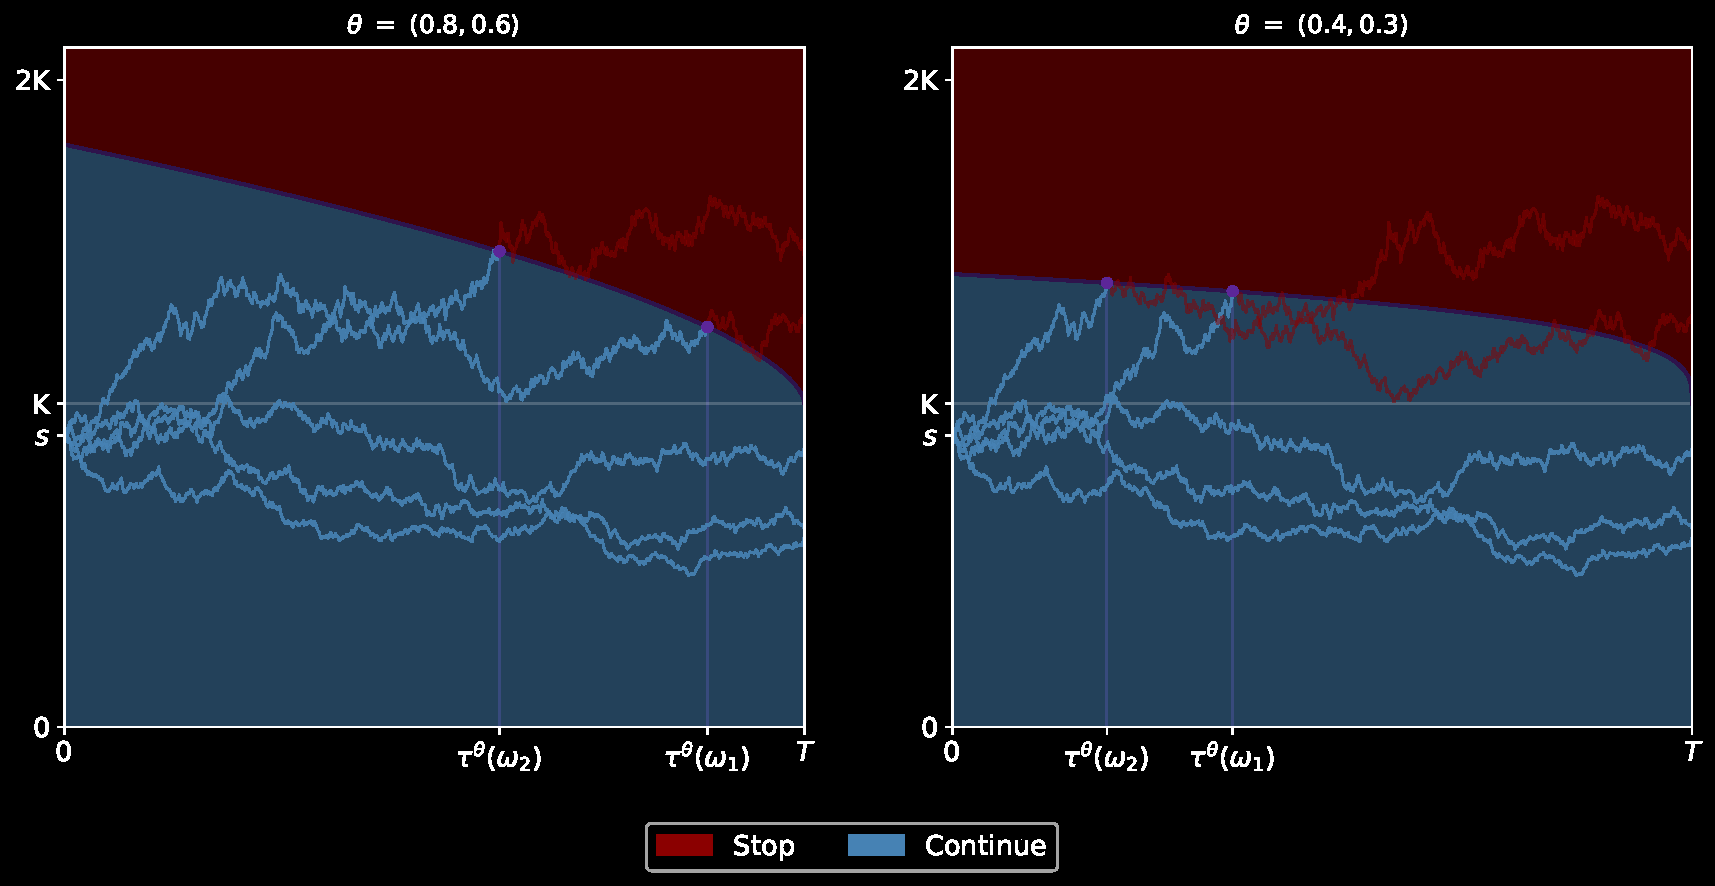
\includegraphics[scale=0.5]{FB/Figures/twoParams.pdf}
     \caption{Boundaries obtained from the two-parameter family $\eqref{eq:twoParams}$.}
     \label{fig:twoParams}
 \end{figure}
 
 

 
 
 
 %In the numerical examples, we will show how neural networks can be employed to parametrize the threshold function. 
 
 %\subsection{Motivation in the one-dimensional case}
